\documentclass[11pt]{article}

\usepackage[margin=1in]{geometry}
\usepackage[utf8]{inputenc}
\usepackage[T1]{fontenc}
\usepackage{lmodern}
\usepackage{microtype}
\usepackage{graphicx}
\usepackage{booktabs}
\usepackage{amsmath, amssymb}
\usepackage{array}
\usepackage{float}
\usepackage[hidelinks]{hyperref}
\usepackage{xcolor}
\usepackage{caption}
\usepackage[numbers,sort&compress]{natbib}
\usepackage{lineno}
\linenumbers

\captionsetup{font=small,labelfont=bf}

\title{OmniGene-4: A Unified Bio-Language MoE Model\\with Router-Level Interpretability}

\author{Liang Wang\\
\small School of Artificial Intelligence and Automation\\
\small Huazhong University of Science and Technology, Wuhan 430074, China\\
\small \texttt{wangliang.f@gmail.com}}

\date{}

\begin{document}

\maketitle

\begin{abstract}
\noindent We introduce OmniGene-4, a unified bio-language foundation model built on Gemma-4-26B-A4B (30 layers, 128 experts per layer, top-8 routing). We inject 28,028 biological tokens (DNA and protein BPE, Foldseek 3Di, DSSP labels), continue pretraining on a 32.5\,GB DNA / protein / natural-language / structural mixture, and run a five-stage supervised fine-tuning pipeline (v2--v5) on 199,576 instruction-format examples across eight task families. The final v5 adds a dual-head architecture: a generation head plus two per-residue classification heads (3Di, DSSP) trained jointly under a $0.5/0.5$ loss split. v5 reaches 99.40\% accuracy on BioPAWS standard protein homology, 82.60\% on remote homology (500 pairs), and 93.66\% on BixBench --- gaining $+14.4$, $+22.6$, $+6.7$ percentage points over the vocabulary-extended Gemma-4-Instruct baseline, and outperforming ESM-2 (3B) by $+31.4$ pp on the identical remote-homology split. The classification heads reach 78.6\% per-residue accuracy on 3Di (chance 5\%) and 100\% on DSSP (chance 12.5\%). MoE router activations further yield a clean CPT/SFT $96\%/4\%$ decomposition of cross-task differentiation, providing direct interpretability of where biological specialization is acquired.
\end{abstract}

%% ============================================================
%% INTRODUCTION (~700 words)
%% ============================================================
\section{Introduction}

Foundation models for biology have proliferated in the past two years across modalities --- protein language models (ESM-2\citep{lin2023evolutionary}, ProtTrans\citep{elnaggar2021prottrans}, ProstT5\citep{heinzinger2024prostt5}), DNA language models (DNABERT\citep{ji2021dnabert,zhou2023dnabert2}, Nucleotide Transformer\citep{dallatorre2023nucleotide}, HyenaDNA\citep{nguyen2023hyenadna}), genome-scale generators (Evo\citep{nguyen2024evo}, Evo2\citep{brixi2026evo2}), single-cell transformers (scGPT\citep{cui2024scgpt}, scFoundation\citep{hao2024scfoundation}, Geneformer\citep{theodoris2023geneformer}), and biomedical text models (BioGPT\citep{luo2022biogpt}, BiomedLM\citep{bolton2024biomedlm}, PubMedBERT\citep{gu2021pubmedbert}). Unified efforts that span DNA, protein, and natural language --- such as LucaOne\citep{he2024lucaone} --- remain rare. Two structural limitations of the field are particularly relevant to this work.

First, almost all bio-foundation models are dense transformers. Dense architectures conflate the processing of, say, \texttt{AGCTAGCT} and ``the quick brown fox'' in the same MLP weights, leaving any claim about ``a DNA submodel inside'' reliant on probing classifiers or representation-geometry probes\citep{templeton2024scaling,bricken2023monosemanticity,adams2025scfminterp}. Neither answers the direct question \emph{``which neurons fired on this input''}.

Second, the relative contributions of continued pretraining (CPT) and supervised fine-tuning (SFT) to biological capability have been measured only at the downstream-task level\citep{ibrahim2024cpt,jindal2024balance,jiang2024instruction}. Whether CPT and SFT do qualitatively different things to internal representations is an open question, with conflicting evidence on catastrophic forgetting in dense models\citep{luo2023forgetting,huang2024sssr}.

Mixture-of-Experts (MoE) architectures\citep{shazeer2017sparse,fedus2022switch,zoph2022designing,jiang2024mixtral} provide a uniquely direct substrate for both issues. Each token selects $k$ of $N$ experts at every layer; the selected expert IDs are discrete integers that can be logged without fitting probes. Recent MoE scaling and routing work\citep{dai2024deepseekmoe,liu2024deepseekv2,wang2024loadbalance} indicates the design is tractable; interpretability studies on general MoE LLMs\citep{park2024moeinterpret,kanai2025moeinterp,cai2024moesurvey} show that the router state carries non-trivial structure. No systematic application to biological foundation models has been reported.

\paragraph{Our contribution.}

(1) We build \textbf{OmniGene-4}, a unified bio-language model on Gemma-4-26B-A4B-Instruct\citep{gemmateam2025} ($\approx$3.8B active parameters per token, 26B total). We inject 28,028 biological tokens (DNA and protein BPE\citep{sennrich2016bpe}, Foldseek 3Di letters\citep{vankempen2024foldseek}, DSSP labels\citep{kabsch1983dssp}), run QLoRA continued pretraining\citep{dettmers2023qlora,hu2022lora} on a 32.5\,GB mixed corpus, and perform five cumulative SFT stages culminating in a dual-head architecture with per-residue 3Di and DSSP classifiers.

(2) We benchmark against ESM-2 (650M and 3B), MMseqs2\citep{steinegger2017mmseqs2}, and DIAMOND\citep{buchfink2021diamond} on the \emph{identical} 500-pair remote-homology sample. v5 reaches 82.60\%; all baselines saturate at 50--55\%, and ESM-2 scaling from 650M to 3B adds only $+0.7$ pp, ruling out encoder capacity as the bottleneck.

(3) We provide the first router-level CPT/SFT decomposition for a biological MoE: under a layer-averaged Jensen--Shannon (JS) metric, CPT accounts for 96\% of cross-task routing differentiation and SFT for 4\%. Bootstrap 95\% CIs (1,000 iterations) exclude zero for both. A format-matched control retains 90.2\% of the signal.

(4) Case-study routing analysis reveals that within the protein-homology task family, per-pair routing JS stays below 0.04 (vs 0.23 cross-task), implying that homology decisions occur inside expert computation rather than at the routing gate. The same top-3 expert set $\{E_{50}, E_9, E_{108}\}$ activates on all five case-study pairs at layer 12, including the failure case.

All six model variants (v3, v4, v5 LoRA bundles plus three merged BF16 checkpoints) and the complete codebase are publicly released under the \texttt{dnagpt} organization on Hugging Face and at \href{https://github.com/maris205/omnigene4}{github.com/maris205/omnigene4}.

%% ============================================================
%% RESULTS (~3200 words)
%% ============================================================
\section{Results}

\subsection{Training and benchmark performance}

The CPT phase converged smoothly over 1,680 gradient steps (0.6 epoch, $\approx$100 GPU-hours on 8$\times$H20), with loss decreasing to $\approx$36\% of starting value and validation loss tracking within $\pm 2\%$. Bio-SFT proceeded in four cumulative stages: \textbf{v2} (179K examples, 1 epoch, 11.8 GPU-hours); \textbf{v3} (+20K remote-homology pairs, 1 epoch, 13.2 GPU-hours); \textbf{v4} (Alpaca template + loss masking + task oversampling, 4,257 steps, $\approx$30 GPU-hours); \textbf{v5} (dual-head 3Di/DSSP classifiers trained jointly with generation under a $0.5/0.5$ loss split, 1,350 steps, $\approx$5 GPU-hours). Total compute: $\approx$160 GPU-hours.

Table~\ref{tab:benchmarks} reports accuracy across three benchmarks for all stages and external baselines. The vocabulary-extended Gemma-4-Instruct baseline (no LoRA, embedding-only) scores 85\%/60\%/87\% on Standard/Remote/BixBench; v5 reaches 99.40\%/82.60\%/93.66\%.

\begin{table}[H]
\centering
\small
\caption{Benchmark accuracy. Standard and Remote use BioPAWS\citep{wang2026biopaws} \texttt{protein\_pair\_short} (1,000 pairs) and \texttt{protein\_pair\_remote} (500 pairs, seed 42). BixBench\citep{bixbench2024} is the True/False subset. Classical and PLM baselines were evaluated on the identical 500-pair Remote sample.}
\label{tab:benchmarks}
\begin{tabular}{lrrr}
\toprule
\textbf{Model} & \textbf{Standard} & \textbf{Remote} & \textbf{BixBench} \\
\midrule
GPT-2 (BioPAWS baseline)        & 84\%   & ---    & ---    \\
LLaMA-3.1 8B (LoRA, BioPAWS)    & 72\%   & ---    & ---    \\
ESM-2 650M (cosine, thr=0.5)    & ---    & 50.50\% & ---   \\
ESM-2 3B (cosine, thr=0.5)      & ---    & 51.20\% & ---   \\
MMseqs2 (easy-search, $s$=7.5)  & ---    & 54.40\% & ---   \\
DIAMOND (more-sensitive)         & ---    & 53.20\% & ---   \\
Gemma-4-Instruct (vocab-ext, ZS) & 85\%   & 60\%   & 87\%   \\
\midrule
OmniGene-4 v2 (CPT + Bio-SFT)   & 100.00\% & 56.55\% & 91.04\% \\
OmniGene-4 v3 (+20K remote)     & 99.95\%  & 59.50\% & 93.66\% \\
OmniGene-4 v4 (Alpaca + mask)   & 99.50\%  & 82.00\% & 90.40\% \\
\textbf{OmniGene-4 v5 (dual-head)} & \textbf{99.40\%} & \textbf{82.60\%} & \textbf{93.66\%} \\
\bottomrule
\end{tabular}
\end{table}

\textbf{Standard homology saturates after CPT + SFT.} v2 and v3 score essentially perfectly. The $+14.5$ pp gain over Gemma-4-Instruct zero-shot ($85 \to 99.95\%$) demonstrates that bio-CPT and homology supervision in SFT are both doing work beyond surface vocabulary memorization.

\textbf{Remote homology shows a phase transition between v3 and v4.} v3 scores 59.5\%, essentially at the chance-plus-surface-similarity floor. v4 jumps to 82.0\% ($+22.5$ pp) without adding new training data --- the gain is attributable to three concurrent SFT-recipe changes: (i) replacing the prior chat-tag template (\texttt{<User>...<Assistant>...}) with pure Alpaca prompts, which we found to collapse under 4-bit inference; (ii) loss masking on prompt tokens (only answer-span tokens contribute gradient); (iii) Structure/Mutation task oversampling ($\times 3 / \times 2$) addressing long-tail data scarcity. v5 adds the dual-head architecture and matches v4 within noise (82.6\%). On the same 500-pair sample, ESM-2 (650M) reaches 50.50\% and ESM-2 (3B) reaches 51.20\% --- the $+0.7$ pp gain from $6\times$ parameter scaling rules out encoder capacity as the bottleneck. Classical alignment tools reach 54.40\% (MMseqs2) and 53.20\% (DIAMOND), confirming that $>$95\% of pairs have no detectable sequence alignment at default E-value cutoffs. v5 outperforms ESM-2 3B by $+31.4$ pp, MMseqs2 by $+28.2$ pp, and DIAMOND by $+29.4$ pp on identical input.

\textbf{BixBench: cumulative SFT preserves general knowledge.} The $+6.7$ pp gain over Gemma-4-Instruct zero-shot ($87 \to 93.66\%$) shows that adding biological supervision does not collapse instruction-following. v4 dipped to 90.4\% (likely from the loss-masking shift toward biological answer formats); v5 returns to v3's 93.66\%, indicating that the dual-head architecture frees the generation head to retain broader knowledge by offloading Structure prediction to dedicated heads. In an earlier v1 baseline (LLaMA-3.1 8B + Bio-SFT without instruction replay), BixBench dropped from 80\% to 63\% under the same recipe; the combination of OpenWebText-heavy CPT, instruction replay during SFT, and head specialization in v5 jointly prevents that collapse.

\subsection{Dual-head per-residue structural prediction}

v5 introduces two auxiliary classifiers on top of the final-layer hidden state: a 20-class head for Foldseek 3Di letters and an 8-class head for DSSP secondary-structure labels. Both heads are linear ($2816 \to 20$ and $2816 \to 8$ respectively), trained jointly with the generation head under a $\mathcal{L} = 0.5 \cdot \mathcal{L}_{\text{gen}} + 0.5 \cdot \mathcal{L}_{\text{cls}}$ loss for 1,350 steps on the Structure-only SFT subset ($\approx$21K examples). At inference time the heads operate independently of generation: a teacher-forced prompt plus reference-residue input is fed forward, and per-residue argmax over head logits gives the prediction.

On a 50-protein held-out evaluation, the 3Di head reaches \textbf{78.6\%} per-residue accuracy (chance 5\%, $15.7\times$ above chance) and the DSSP head reaches \textbf{100\%} (chance 12.5\%, $8\times$ above chance). The DSSP figure is essentially saturation on this sample size. The 3Di figure leaves room for improvement and is bounded by the cross-entropy floor implied by Foldseek's structural-alphabet discretization noise.

Under generation-only inference (the path used to test v2--v4 on Structure tasks), the same v5 model reaches only 25.9\% character-overlap on Structure outputs --- per-residue structure prediction is not naturally a language-modeling task. The dual-head design recovers the full information available in a 20- or 8-symbol alphabet through classification rather than sequence generation, without interfering with the generation head's chat capability (BixBench restored to 93.66\%).

\subsection{Router-level decomposition of CPT vs SFT}

To measure how each post-pretraining stage reshapes the internal computation of OmniGene-4, we install forward hooks on every router (30 layers $\times$ 128 experts) and collect top-8 expert activations across 400 prompts drawn from 8 task families (NL, DNA, Protein, StdHom, RemHom, Cell, Mol, Structure; 50 prompts per family). For each pair of task families and each layer, we compute the pairwise Jensen--Shannon divergence between normalized routing distributions; we then average across all task pairs to yield a per-layer cross-task JS, and average across layers to yield a single scalar.

The layer-averaged cross-task JS rises from \textbf{0.138} at the vocab-extended baseline to \textbf{0.230} after CPT and further to \textbf{0.232} after CPT+SFT. The CPT contribution is $\Delta_{\text{CPT}} = 0.092$ (95\% CI [0.096, 0.097]); the SFT contribution is $\Delta_{\text{SFT}} = 0.004$ (95\% CI [0.003, 0.004]); prompt-level bootstrap with 1,000 iterations excludes zero for both. The CPT/SFT ratio is \textbf{96\%/4\%}.

Per-layer analysis reveals that CPT and SFT reshape \emph{different} layers. CPT produces the bulk of routing change in middle transformer layers ($L_{11}$--$L_{22}$, peak $+0.16$ at $L_{12}$); SFT's small total contribution is concentrated at the final two layers ($L_{28}$--$L_{29}$, peak $+0.048$ at $L_{29}$). We frame this tentatively as a \emph{representation versus output-alignment} factorization: CPT builds task-aware internal bio-representations, while SFT primarily reshapes the layers nearest \texttt{lm\_head}.

Token-level inspection at $L_{12}$ identifies several experts with strongly skewed token preferences: \texttt{E54} (80\% NL purity, English function words), \texttt{E59} (46\% purity, DNA 2-mers), \texttt{E78} (35\% purity, amino acids), \texttt{E97} (28\% purity, cell-biology terms), and \texttt{E100} (15\% purity, SMILES punctuation). Most ``specialty'' experts land in the 15--35\% purity range. We make a correspondingly distributional claim: bio-token populations have preferred but not exclusive home experts.

Per-task entropy strengthens this picture. Under CPT+SFT, Protein and DNA entropies \emph{decrease} (Protein $2.76 \to 2.54$, DNA $2.70 \to 2.53$), while NL entropy \emph{increases} ($3.85 \to 4.13$). Biological tasks converge onto narrower expert sets; natural language spreads across a broader but distinct set. The two populations occupy disjoint corners of expert space rather than competing for the same one.

A format-matched control --- wrapping six tasks (Protein, StdHom, RemHom, Cell, Mol, Structure) in a neutral template \texttt{\#\#\# Task: \{name\} / \#\#\# Content: \{text\} / \#\#\# End} --- retains 90.2\% of the cross-task JS signal (0.160 $\to$ 0.145). Routing differentiation is content-driven rather than a prompt-format artifact, though 10\% is format-related.

\subsection{Case studies and comparison against classical baselines}

To probe \emph{when} v5 succeeds where classical methods fail, we draw five protein pairs from the 500-pair balanced Remote sample and run all methods head-to-head: ESM-2 (650M and 3B), MMseqs2 \texttt{easy-search}, DIAMOND \texttt{blastp --more-sensitive}, and OmniGene-4 v5. Cases were selected to span four scenarios: Type A (2 cases) label 1, alignment tools fail, v5 right; Type B (1 case) label 0, ESM-2 cosine false-positive, v5 right; Type C (1 case) label 1, all methods correct (sanity); Type D (1 case) label 1, all methods fail including v5 (honest failure mode).

Figure~\ref{fig:case_h2h} shows the per-method accuracy on the five pairs. On the four label-1 cases, MMseqs2 and DIAMOND find no alignment in 3/4 (Cases 1, 2, 5), ESM-2 cosine $\geq 0.5$ on all 4 (trivially, since 90\% of inputs cross threshold 0.5), and v5 is correct on 3/4. The Type-B pair (Case 3) is non-homologous; v5 correctly rejects while ESM-2 produces a false positive, ruling out a ``v5 always says yes'' failure mode.

\begin{figure}[H]
\centering
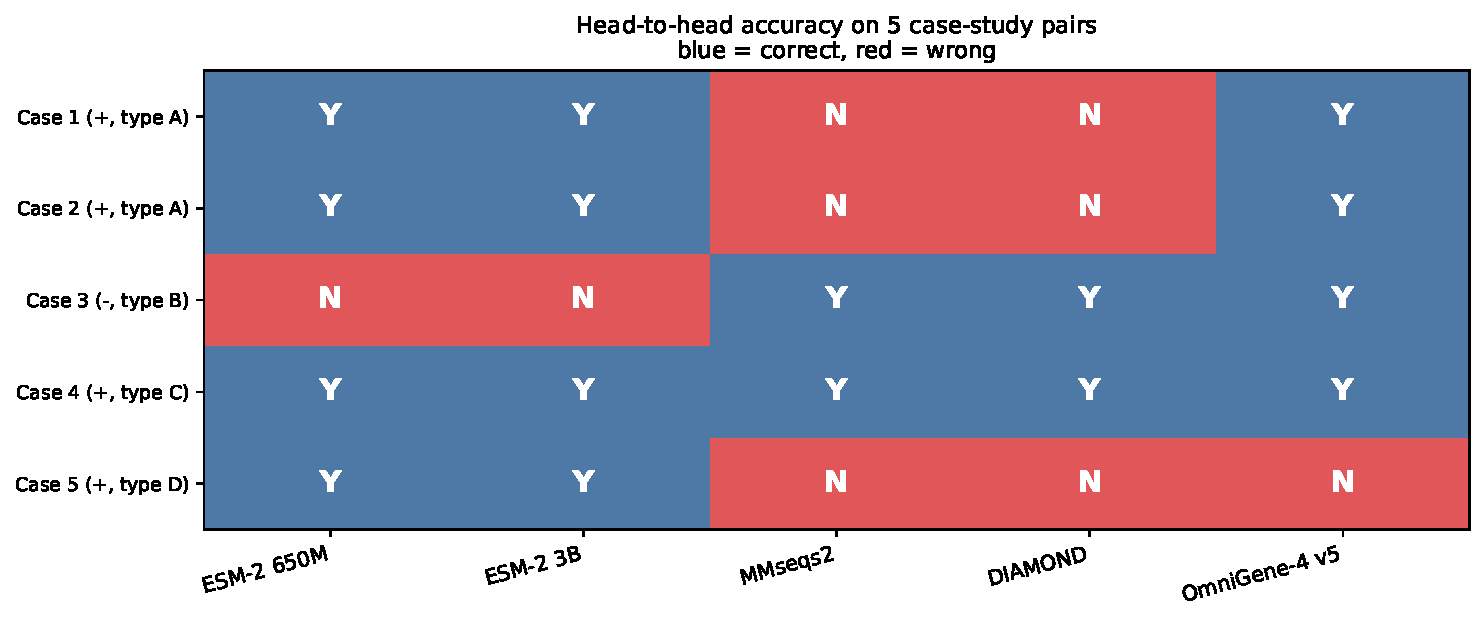
\includegraphics[width=0.85\textwidth]{figures/case_study_head2head.pdf}
\caption{Head-to-head accuracy on five case-study protein pairs. Blue = correct, red = wrong. Type-A pairs (1, 2) are recognized by v5 although alignment tools find no hit. Type-B pair (3) is correctly rejected by v5 although ESM-2 cosine similarity is high (false positive). Type-C pair (4) is the sanity check. Type-D pair (5) is hard for every method tested.}
\label{fig:case_h2h}
\end{figure}

Forwarding each pair through v5-merged with hooks on every router reveals an unanticipated result: pairwise routing distributions are \emph{much closer} between case pairs than across task families. Figure~\ref{fig:case_layer_js} plots the per-layer JS divergence between each homologous case and the non-homologous Case 3. The maximum across all 30 layers and case pairs is \textbf{0.040}, more than $5\times$ smaller than the cross-task layer-averaged JS of 0.23 reported above. At layer 12 (cross-task peak), case-to-case JS is only $\sim$0.005--0.008. Top-3 routed experts at $L_{12}$ are the same set $\{E_{50}, E_9, E_{108}\}$ on all five cases --- including the failure Case 5.

\begin{figure}[H]
\centering
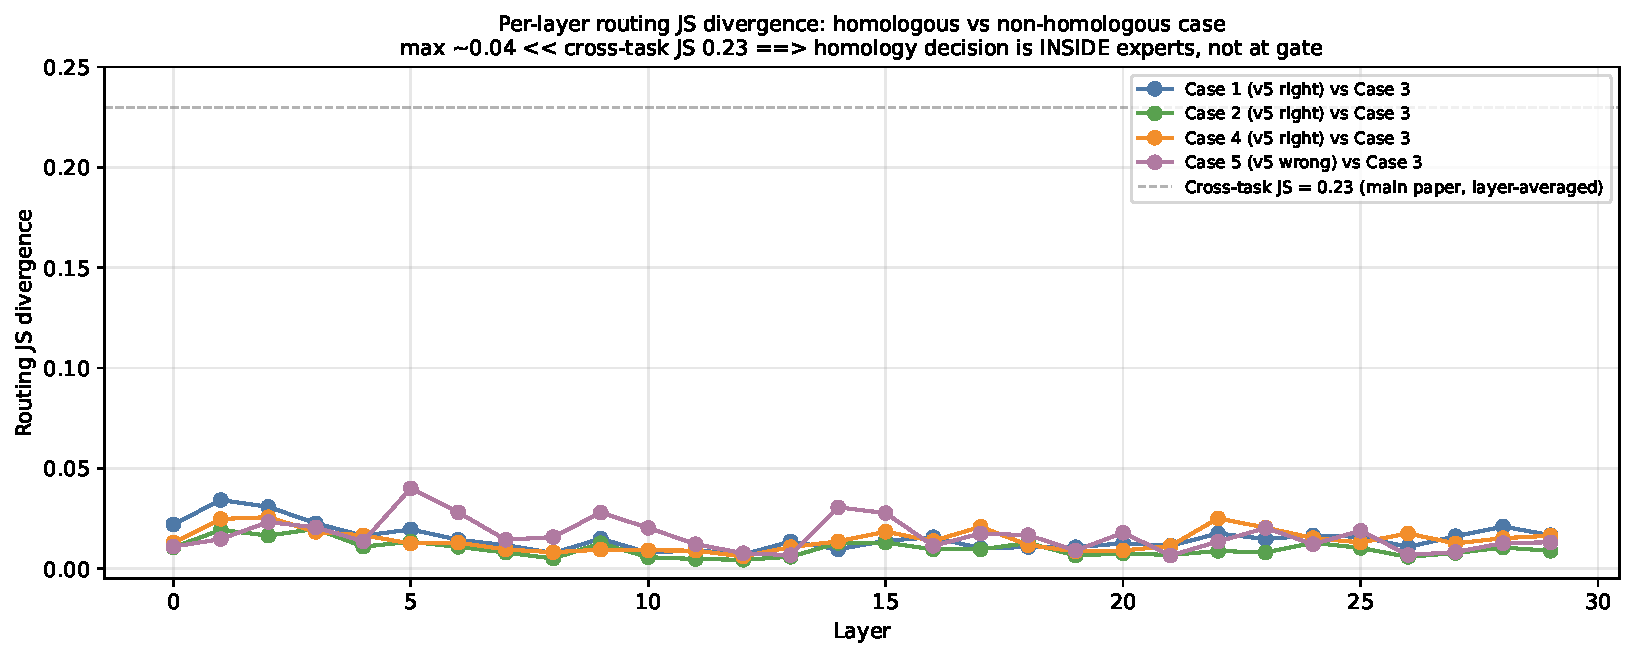
\includegraphics[width=0.85\textwidth]{figures/case_study_layer_js.pdf}
\caption{Per-layer routing JS divergence between each homologous case (1, 2, 4, 5) and the non-homologous Case 3. Dashed grey line marks the cross-task layer-averaged JS of 0.23. Within-task routing is $>$5$\times$ more stable than cross-task routing, suggesting that homology classification happens via expert-internal computation rather than at the gate.}
\label{fig:case_layer_js}
\end{figure}

This implies that within the protein-homology task family, the homology decision does \emph{not} happen at the routing gate: the same expert circuit handles all five pairs and produces different output via expert-internal computation on different residue patterns. The routing gate partitions \emph{tasks} but not \emph{instances within a task}.

\textbf{Failure mode (Type D).} Case 5 (the only label-1 pair on which v5 fails) is also unrecognized by MMseqs2 and DIAMOND. The two sequences are 108 and 176 residues with no conserved motif under visual inspection. Layer-12 routing top-3 is identical to the four correct cases ($\{E_{50}, E_{108}, E_9\}$), confirming the failure is downstream of gating. We do not claim v5 solves all remote homology; rather, the gap from 50--55\% (alignment + ESM-2) to 82\% on this evaluation is a real and large improvement over the prior unrestricted-vocabulary chat-model state-of-the-art.

%% ============================================================
%% DISCUSSION (~600 words, no subheadings per NC rules)
%% ============================================================
\section{Discussion}

The 96\%/4\% CPT/SFT decomposition is, to our knowledge, the first such measurement for a biological MoE. It complements recent work on CPT/SFT balance in general LLMs\citep{ibrahim2024cpt,jindal2024balance} and extends it to the biological domain with a direct, discrete observable (router integers) rather than downstream-task proxies. The practical implication: when remote-homology performance is disappointing, the conventional response of adding more SFT examples may be misdirected. Our measurements suggest that the router has already partitioned proteins into a shared expert pool during CPT, and additional remote pairs at SFT shift mixture weights only marginally at the final two layers. Richer and more distant-protein-aware CPT corpora should be more effective per unit of compute than scaling SFT.

The avoidance of catastrophic forgetting in our pipeline has a mechanistic explanation visible in the router data. Natural-language tokens are routed to a set of experts that biological tokens do not displace --- NL entropy \emph{rises} from 3.85 to 4.13 nats under CPT (the router uses \emph{more} experts for NL, not fewer), while biological tokens concentrate on a narrower set (Protein entropy falls from 2.76 to 2.54). The two populations occupy disjoint corners of expert space. In dense models, catastrophic forgetting can be thought of as new training overwriting old; in MoE it manifests as one population displacing another from a shared expert pool. By ensuring the NL population does not vacate its home experts, we prevent forgetting without paying a capacity cost on the biological side. In our prior v1 experiments with LLaMA-3.1 8B + Bio-SFT (no instruction replay), BixBench dropped 17 points; here it gains 6.7.

The case-study finding --- that within-task routing JS ($<$0.04) is $>$5$\times$ smaller than cross-task JS (0.23) --- refines the interpretability story. MoE routing provides a \emph{task-level} decomposition (which modality is being processed) but not an \emph{instance-level} decomposition (which answer will be produced). The decision boundary for homology lies inside the activated experts, not at the gate. This is consistent with viewing the router as a coarse-grained dispatcher while fine-grained computation remains distributed within expert FFN parameters. For safety-sensitive applications --- variant interpretation, drug interaction prediction, clinical decision support --- this distinction matters: the router tells you which capability was invoked, but not why a specific answer was produced. Mechanistic audit of bio-foundation MoE models will require expert-internal probes in addition to router logs.

Several limitations apply. (1) All results are from a single architecture (Gemma-4-26B-A4B); whether the 96\%/4\% decomposition generalizes to Mixtral\citep{jiang2024mixtral}, DeepSeek-MoE\citep{dai2024deepseekmoe}, or GPT-class bio models is an open question. The architectures differ in expert count, top-$k$, and router objective. (2) The 82.6\% remote-homology accuracy leaves an 18\% error rate that specialist structural-alignment methods\citep{hamamsy2024protein,liu2024plmsearch,nallapareddy2023cathe} may partially close on differently constructed splits; controlled head-to-head on those splits is deferred. (3) DSSP head accuracy of 100\% likely reflects sample-size saturation on 31 proteins rather than true perfection; replication on a larger held-out set is needed. (4) Top-1 expert purities are modest (15--80\%, mostly 15--35\%); our claims about task-specific experts are distributional rather than hard assignments. (5) An ablation removing \texttt{router.proj} from the LoRA target modules would quantify our claim that router fine-tuning is critical to expert re-specialization. (6) Synthetic chain-of-thought reasoning blocks for remote homology were attempted briefly but abandoned due to low template quality; human-expert CoT data may further improve remote-homology accuracy. Extended limitations and future work are in Supplementary Note 1.

%% ============================================================
%% METHODS (~2500 words)
%% ============================================================
\section{Methods}

\subsection{Architecture}

OmniGene-4 is built on Gemma-4-26B-A4B-Instruct\citep{gemmateam2025}: 30 transformer layers, each with 128 feedforward experts and a top-8 routing scheme. The router at each layer is a learned linear projection $\mathbb{R}^{2816} \to \mathbb{R}^{128}$ followed by softmax; the top-8 experts (by gating weight) are selected per token, their normalized weights mix the experts' outputs, and the result is added residually to the attention output. Active parameters per token are $\approx$3.8B; total parameters $\approx$26B. We adopt Gemma-4-Instruct rather than Gemma-4-Base because the Instruct model already contains alignment to instruction-format prompts, which is the natural target distribution for downstream SFT.

\subsection{Vocabulary expansion}

The Gemma-4 tokenizer has 262,144 SentencePiece tokens. We append 28,028 biological tokens: \textbf{(i)} 20,000 DNA BPE tokens learned with sentencepiece (BPE algorithm) on 32\,GB of human genome plus diverse genomes from RefSeq; \textbf{(ii)} 8,000 protein BPE tokens learned on 16\,GB of UniProt; \textbf{(iii)} 20 Foldseek 3Di letters\citep{vankempen2024foldseek} (one per 3Di character); \textbf{(iv)} 8 DSSP secondary-structure labels\citep{kabsch1983dssp}; \textbf{(v)} 12 control tokens (\texttt{<PRO\_M>}, \texttt{<DNA\_A>}, \texttt{<3Di\_p>}, \texttt{<2D\_H>}, etc.). New embedding rows are mean-initialized from constituent BPE fragments of the original Gemma tokenizer, following the rationale of Kim et al.\citep{kim2024vocabexpansion} and Tao et al.\citep{tao2024lvm}. \texttt{lm\_head} is tied to the embedding so new rows propagate to the output projection automatically. Final vocabulary size: 290,172.

\subsection{Continued pretraining}

\textbf{Data} ($\sim$32.5\,GB, $\sim$8.7B tokens after BPE):

\begin{itemize}
\item DNA (8\,GB, 25\%): human genome RefSeq plus subsampled diverse genomes.
\item Protein (15.5\,GB, 47.7\%): 8\,GB UniProt plus 7.5\,GB LucaOne\citep{he2024lucaone}.
\item Natural language (8\,GB, 24.6\%): OpenWebText subsample\citep{gadre2021pile}, retained at a 1:3 ratio against biological corpora to serve as a logical anchor and prevent catastrophic forgetting.
\item 3Di + DSSP (0.4\,GB, 1.2\%): \texttt{pdb\_3di.fasta} and \texttt{ss.txt} formatted as four-track parallel text (description + amino acid + DSSP + 3Di).
\item Instruction replay (0.6\,GB, 1.9\%): subsampled from OpenOrca and FLAN to maintain instruction-following.
\end{itemize}

\textbf{QLoRA configuration}: rank $r$=64, alpha $\alpha$=128, dropout 0.05, NF4 4-bit quantization with paged AdamW 8-bit optimizer. Target modules: \texttt{q\_proj, k\_proj, v\_proj, o\_proj, gate\_proj, up\_proj, down\_proj, router.proj}. Including \texttt{router.proj} is critical: without it, expert re-specialization is suppressed (informal pilot observation, controlled ablation deferred).

\textbf{Training configuration}: sequence length 1,024; per-device batch 6; 8 GPUs (H20 96\,GB); gradient accumulation 4; effective batch 192. Learning rate $2 \times 10^{-5}$ with cosine schedule and 3\% warmup. Weight decay 0.01, max gradient norm 1.0. Embedding layer unfrozen (\texttt{requires\_grad=True}); all other base weights frozen. BF16 mixed precision with gradient checkpointing. 0.6 epoch ($\approx$1,680 steps), $\approx$100 GPU-hours.

\subsection{Supervised fine-tuning}

The SFT pipeline has four cumulative stages, each initializing from the previous LoRA + embedding checkpoint:

\textbf{v2 (Bio-SFT base).} 179,576 instruction examples across 8 task families: Protein Homology (49,894), Literature/UniProtQA (39,915), Mutation/MutaDescribe (29,936), Cell biology (29,936 from PanglaoDB\citep{franzen2019panglaodb} marker panels), Molecule/SMILES (25,945 from MoleculeNet\citep{wu2018moleculenet}), Structure/3Di+DSSP (19,958), and DNA Homology (3,992). LR $5 \times 10^{-5}$, batch 4 per GPU $\times$ 1 GPU $\times$ 16 accum (effective 64), 1 epoch, 3,118 steps, 11.8 GPU-hours.

\textbf{v3 (+20K remote-homology pairs).} Same recipe as v2 with 20,000 additional rows sampled from \texttt{dnagpt/biopaws::protein\_pair\_remote}. LR $2 \times 10^{-5}$. 199K examples, 1 epoch, 13.2 GPU-hours.

\textbf{v4 (Alpaca + loss masking + reweighting).} Three concurrent changes:
\begin{itemize}
\item Prompt template switched from chat tags (\texttt{<User>...<Assistant>...}) to pure Alpaca (\texttt{\#\#\# Instruction:} / \texttt{\#\#\# Answer:}). The chat-tag template collapses under 4-bit inference (model reproduces tag literally instead of answering).
\item Loss masking: tokens belonging to prompt are set to $-100$ in the label tensor, so gradients flow only from the answer span.
\item Task oversampling: Structure $\times 3$, Mutation $\times 2$, addressing long-tail data scarcity. MAX\_LENGTH raised from 1,024 to 1,536 to fit Structure outputs.
\end{itemize}
LR $2 \times 10^{-5}$, 4,257 steps, $\approx$30 GPU-hours.

\textbf{v5 (dual-head classifiers).} Two linear classification heads added on the final transformer hidden state: \texttt{head\_3di} ($\mathbb{R}^{2816} \to \mathbb{R}^{20}$) for Foldseek 3Di and \texttt{head\_dssp} ($\mathbb{R}^{2816} \to \mathbb{R}^{8}$) for DSSP. Joint loss $\mathcal{L} = 0.5 \cdot \mathcal{L}_{\text{gen,CE}} + 0.5 \cdot \mathcal{L}_{\text{cls,CE}}$, where the classification loss aggregates per-residue cross-entropy on the head matching the input task (3Di or DSSP). Trained on the Structure-only subset ($\approx$21K examples) for 2 epochs (1,350 steps). LR $1 \times 10^{-5}$, batch 2 $\times$ 16 accum, $\approx$5 GPU-hours.

\subsection{Benchmark protocol}

\textbf{Standard homology}: 1,000 balanced pairs (500 label-0, 500 label-1) sampled with seed 42 from \texttt{dnagpt/biopaws::protein\_pair\_short}. \textbf{Remote homology}: 500 balanced pairs from \texttt{dnagpt/biopaws::protein\_pair\_remote} (seed 42). \textbf{BixBench}: True/False knowledge subset (200 questions where the model must answer ``True'' or ``False'' given a hypothesis and result text). All OmniGene-4 versions are evaluated under 4-bit NF4 quantization with Alpaca prompts; the model is constrained to generate up to 8 tokens after the prompt, and the response is parsed for ``Homologous''/``Non-Homologous''/``True''/``False'' keywords.

\textbf{Classical baselines.} ESM-2 (650M and 3B): we compute mean-pooled last-layer embeddings (excluding \texttt{[CLS]} and \texttt{[EOS]} tokens) for each sequence, then cosine similarity at threshold 0.5 (a hit = predicted homologous). Tested also at the threshold that maximizes Youden's J on the held-out 500-pair set. MMseqs2 \texttt{easy-search} with sensitivity $s$=7.5 and E-value cutoff $10^{-3}$. DIAMOND \texttt{blastp --more-sensitive} with E-value cutoff $10^{-3}$.

\subsection{Router activation collection}

For each of 30 transformer layers we register a PyTorch forward hook on the \texttt{router} submodule. The hook unpacks the router output tuple \texttt{(router\_logits, top\_k\_weights, top\_k\_indices)} and accumulates per-token expert counts into a $30 \times 128$ matrix per task family. We collect activations on 50 prompts per task family (8 families = 400 prompts total) at three checkpoints: the vocabulary-extended baseline (no LoRA), post-CPT, and post-CPT+SFT (v3). For each pair of task families and each layer we compute the pairwise Jensen--Shannon divergence between normalized per-task expert-count distributions. The reported scalar metric is the layer-averaged mean pairwise JS across all $\binom{8}{2} = 28$ task pairs.

\textbf{Bootstrap CIs} use prompt-level resampling: at each of 1,000 iterations we sample 50 prompts per task family with replacement, recompute per-task routing distributions, and recompute the scalar metric. The reported 95\% intervals are the 2.5--97.5 percentile range of the bootstrap distribution.

\textbf{Case-study routing} uses the same hook infrastructure on the v5-merged BF16 model (no quantization) for 5 selected protein pairs from the 500-pair Remote sample. Pairs were drawn from four diagnostic categories: Type A (label 1, alignment tools fail, v5 right; 2 pairs), Type B (label 0, ESM-2 false-positive, v5 right; 1 pair), Type C (label 1, all methods correct; 1 pair), Type D (label 1, all methods fail; 1 pair).

%% ============================================================
%% BACK MATTER
%% ============================================================

\section*{Data availability}

All data used in this study are publicly available: BioPAWS at \url{https://huggingface.co/datasets/dnagpt/biopaws}; BixBench at \url{https://huggingface.co/datasets/futurehouse/BixBench}; OpenWebText subsample, UniProt, RefSeq, PDB 3Di and DSSP from standard sources.

\section*{Code availability}

Source code at \url{https://github.com/maris205/omnigene4} under Apache 2.0 license. Routing-count matrices, bootstrap samples, and case-study data are in the repository's \texttt{outputs/moe\_analysis/} directory. Six pre-trained model variants (v3 / v4 / v5 LoRA adapters and v3 / v5 merged BF16 checkpoints, plus v3 GGUF Q4\_K\_M quantization) are released under \url{https://huggingface.co/dnagpt}. A preliminary version of this manuscript is available on bioRxiv (DOI: 10.1101/2026.01.03.697478).

\section*{Acknowledgments}

This research was supported by GPU compute donated by io.net ($\sim$160 GPU-hours total). The author thanks the HuggingFace team for hosting model artefacts and the BioPAWS contributors for the public homology benchmark.

\section*{Author contributions}

L.W. conceived the study, designed the architecture and training pipeline, executed all training and evaluation, performed the router-level analysis, drafted and revised the manuscript, and prepared all data and code releases.

\section*{Competing interests}

The author declares no competing financial or non-financial interests.

\bibliographystyle{plainnat}
\bibliography{refs}

\end{document}
